This part of the exercise has been completed in the attached notebook. The resulting plots will be displayed both here and there:\\
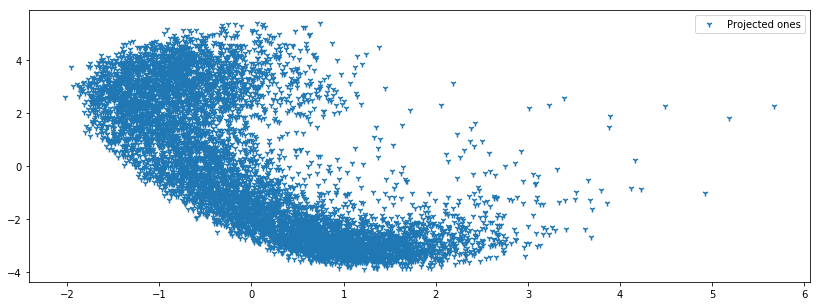
\includegraphics[width=1\linewidth]{3b1.png}
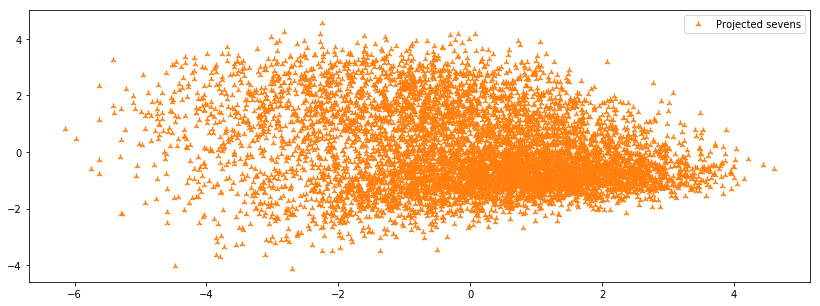
\includegraphics[width=1\linewidth]{3b2.png}
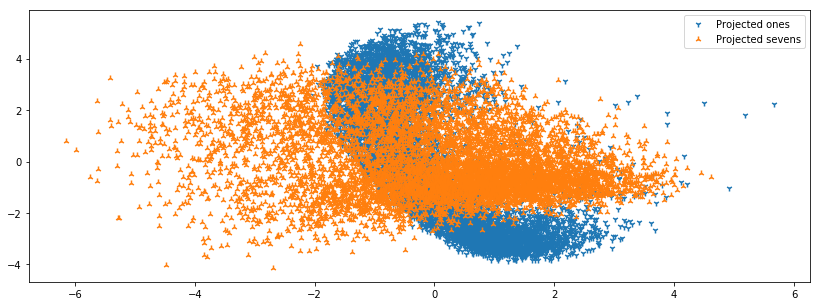
\includegraphics[width=1\linewidth]{3b3.png}\\
We can see from these plots that there is a significantly smaller variance in the "ones" set than in the "sevens" set. This is likely because the difference between the different sevens is larger than between the different ones. Something like the middle line through the seven, and the angle at which you draw it can vary significantly from person to person, whereas the with ones the only significant difference is whether they draw the small tip at the top.\\
The relevant code can be seen here:
\begin{verbatim}
proj1Ones = center(ones) @ eigVecs[:,0]
proj2Ones = center(ones) @ eigVecs[:,1]
proj1Sevens = center(sevens) @ eigVecs[:,0]
proj2Sevens = center(sevens) @ eigVecs[:,1]

plt.scatter(proj1Ones, proj2Ones)
plt.scatter(proj1Sevens, proj2Sevens)
plt.show()
\end{verbatim}